\documentclass[nostrict]{szablonPG}
\usepackage[unicode=true]{hyperref}
\usepackage{pgfplots}
\usepackage{gnuplottex}
\usepackage{graphicx}
\usepackage{mathtools}
\newcommand\PDFtitle{Application of blockchain and infection processes in graphs}
\newcommand\PDFauthors{Stanisław Barański}
\hypersetup{
  pdftitle={\PDFtitle},
  pdfauthor={\PDFauthors},
   pdfsubject={Mitigation Content Posioning},
   pdfkeywords={Content Poisoning, Blockchain, ICN, Graph infection}
 }
 
\usepackage{multicol} 
\makeatletter
\renewcommand{\verbatim@font}{\ttfamily\small}
\makeatother
 
\begin{document}

\tableofcontents
\listoffigures


\begin{abstract}
Information-centric networks introduce new vector of attacks, one of them is content poisoning, which when performed successfully, can create destructive damages. Currently known authentication methods like login/password, private key, biometry, SMS/email confirmation operate on the same dimension of authentication. We propose another dimension of authentication which is time availability. When intruder publisher is operating in time-constrained environment, his access to target identity is limited, whereas honest publisher is not constrained in any way. We leverage such distingshion to propose new authentication mechanism. Two implementations are proposed, first one is based on infection processes in graphs and second one is backed by blockchain technology. 


\end{abstract}


\section{Introduction - State of the art}
Current internet architecture is mostly based on TCP/IP stack, which allow  establish communication channels between two IP addresses. While it worked great for past years,  it struggle to fit current demands. Today internet is dominated by transporting content such as audio, video, images and text[source] from content creators to content consumers. 
https://www.youtube.com/watch?v=8Z685OF-PS8
% Write more about how the internet is used today
% Write more about why current architecture doesn't fit 
% ICN - the solution !!!
The Information-centric networks introduce paradigm shift from host-centric to content-oriented paradigm. Placing content in the center of interest. This allows us to achieve number of benefits. All network participates become more aware of the transferring content. This kind of awareness allows to implement various improvements over host-based paradigm such as content caching, mobility, integrity and security assurance. All of those features are guaranteed naively by ICN transport layer in contrast to TCP/IP where we needed to build them on top of it. There are many implementations of ICNetworks, the most notable:  NDN\cite{zhang2014named}, DONA\cite{koponen2007data} or IPFS \cite{benet2014ipfs}
% continue with Content protection in NDN

\section{IPFS}
"The InterPlanetary File System (IPFS) is a peer-to-peer distributed file system that seeks to connect all computing devices with the same system of files."  \cite{benet2014ipfs} % Can I quote like that ?


\section{NDN}


\section{Content Poisoning - Problem}
The most significant benefit of ICN networks is content caching. It turns out that this benefit becomes double-edged sword when we take into account security concerns. 
First we would like to narrow our interest of research in this paper. Content Poisoning in NDN (and possibly in all ICN networks) can be divided to two categories: 1. Corrupted Data and 2. Fake Data. In both of them the content gets modified. The first one assume that the attacker does not posses the signing-key of legit publisher, thus the content won't pass the signature verifiaction process. This might look like the problem is resolved. Unfortunatelly the signature verifaiction is optional process, and there are two reasons why this process won't be done on every router. First one is the economic incentivisation, the process of signature verification is highly resource-consuming, thus the businesses might decide to skip it. Next reason is based on the fact, that in order to proceed the signature verification, the corresponding public key is required. How can the router know which public key to use? We can not expect from router to store all possible public keys. Thus the routers are vulnerable to Corrupted Data Content-Poisoning Attacks. This kind of attacks has been addressed in many papers \cite{ghali2014needle} \cite{yu2018content} \cite{nguyen2017content}. Second CPA category (Fake Data) is much more dangerous, because it assumes that the Attacker gets access to publisher private-key. Therefore he is able to forge valid signature, which will successfully pass verification on the end-system. 

Once the bogus content gets propagated across multiple nodes (more specifically on their content caches), each end-user who request the content from that node, will receive the poisoned content. Signature verification will pass successfully, hence the user will be sure that the content is legit. What is even worse, the content can not be as easly revoked as it was disseminated, because most of the ICN networks doesn't allow removing/revoking its cache content, other than natural (e.g. LRU based) cache aging. The one way to effectively prevent from fetching fake content is by explicitly filtering the hash of the content we consider poisoned. But this arises another problem, how the user can know the hash of the poisoned content, and if it's not too late. In \cite{nguyen2017content} we can read "Therefore, it (Fake Data CPA) is harder to create but impossible to detect by end-systems". Here it is worth to cite another quote "It always seems impossible until it's done." from Nelson Mandela. At the time of writing, the problem is still unsolved, but there is one proposal \cite{jekon2019content} which we will research, expand and modify. But before that, let's see how other content-oriented services solve the Fake Data CPA problem, in the hope of inspiration.


\subsection{Wikipedia}
Wikipedia is great example of system that face content poisoning problem. Let's investigate how do they solve the problem. 

"Wikipedia is a free online encyclopedia, created and edited by volunteers around the world and hosted by the Wikimedia Foundation."
Everyone can become Wikipedia editor just by creating free account. Account registration doesn't even require email address. Editor can create new article or modify existing one. Before the change is publicly available, other editors read the proposition, and have a chance to reject it or propose further edit. If they can not achieve consensus, they start a discussion where they exchange their arguments, finally if they agree on one version, consensus is achieved and new version of article is published (keeping the whole history of changes).
% What are the kinds of sockpuppeting 
% How to fight with sockpuppeting
% https://en.wikipedia.org/wiki/Wikipedia:Sock_puppetry
% they take into account the 5 phillars  etc. etc.
Such ease of account creation makes Wikipedia vulnerable to Sockpuppeting (also known as Sybil attack). This breach allows one user to create multiple accounts with different identity. In consequence, one person control fake "public opinion", which can support his position in edits discussions. That's why raw voting system is non-preferred method in conflict resolutions. Wikipedia consensus is rather collaborative, in contrast to competition consensus (e.g. used in Bitcoin consensus, where only one account who first find the proof-of-work wins all block reward). 
Wikipedia fight with content poisoning attacks, by using human to detect bogus changes. This mechanism seems to work well in such service, but it doesn't scale to public internet protocol. So we can not use it as is.

\subsection{LOCKSS}
LOCKSS is decentralized p2p digital preservation system. It was build by Standford University for libraries \cite{maniatis2003preserving}. Currently it's open source, decentralized system used by many institutions. Helping them to maintain digital collection of journals, articles, books etc. If we abstract from the specific type of data the system is operating on. We notice that it has some similarities with ICNetworks, that we believe are worth investigation. Main difference between LOCKSS and ICN is the fact that the former is very conservative, it rather prevent, than expedite change of data. But this property may be useful in context of preventing bogus data diffusion. 
In LOCKSS, each participating library becomes a node in p2p network. Node run software that is responsible for collecting new content from e-journal websites by crawler, serving already stored materials to local readers, and cooperating with other nodes in preserving materials when they gets damaged. 
Due to copyrights of publishers, it's important that no node redistribute its content blindly to other peers. Other nodes can help to repair damaged or completely missed materials only to nodes that previously proved the ownership of such content. New materials can only be acquired directly from publisher website to libraries which paid for subscription. 
Damage detection is solved in cyclic polls, where each interested peer, vote on the hash of the storing Archive Unit (smallest unit in which nodes identify each content). Since each node consist of different set of Archive Units (AU), the protocol treat each AU independently. If it turns out that some node contains AU with different hash than majority of the poll, it start sequence of repairs. In result LOCKSS become self-healing store of data, and does not increase risk of free-loading non-purchased content.
LOCKSS is designed in a way that doesn't rely on long-time public-key cryptography. System that must operate for decades, is highly susceptible to eventually private-key leakage. Since it doesn't rely on public-key cryptography, the peer identity is very limited, therefore such system can not rely on peer reputations.

\subsection{Social Media and Fake News}
Fake News is an deliberate disinformative news that is hard to identify, and can lead to descructive consequences if not mitigated on time. Social media are perfect ecosystem for disseminating such kind of content, where the algorithms are designed to serve us the content, that we are likely to agree. In \cite{zhou2018fake} authors point out, why social media algorithms are very effective in fake news dissemination. Social media allow to form a similar minded people into groups, easier than ever before. Such groups facilitate Echo Chamber effect, where each individual is surrounded by people who share and produce content that fits our current world view. This leads to segmented and polarized society, which is very prone to believe in fake news that confirm current opinions, even if there is limited or no reason to believe in such. 

Fake News are written in very provocative fashion, making the content more attractive to interaction, more interaction lead to higher dissemination, which make even more interaction, and so on. While for honest publisher and valuable content this feature is helpful, it becomes very dangerous tool in hands of malicious publishers. Additionally the low cost of creating new accounts makes it even easier for attacker to initiate the snow-ball effect, using fake accounts. Bots can interact with people or even with other bots, creating fake social opinions.  

We notice that this thread model fits perfectly into our Content Posioning Attack model. In some sense, we are facing similar problem Fake News in social media does. We want to allow valuable content to spread as fast as possible, while limiting malicious content dissemination to the minimum.


\subsubsection{How to mitigate fake news}
One idea is to create centralized services, that reveal known fake news. So each time someone is susceptible to some news, he can check if the news in not present in blacklisted news. Although this might seem great solution, it struggle with one significant flaw. Attacker can publish honest news in such "oracle" service, leading to revoking genuine news, which can he as harmful as publishing fake news. A better way would be to check many independent "oracle" services, and evaluate your decision based on how many of them is sceptical to such news.

Another idea would be to create a certification services. Each news could be signed by services who decide that such content is legit or not. The user could decide which certification services he trust, and therefore inherit the trust to the news signed by such services. This idea seems to work for decades in journalism. The reader of reliable journal, does not need to check each article if it's fake or not. He inherit the confidence to each article included the journal, because he trust that the journal's reviewers did the work to eliminate fake, or low quality content. Additionally the journal publisher, has no interest to publish low quality content, because he has economic incentivization to become as creditworthy publisher as possible.
Of course this idea also comes with the downsides. The process of reviewing article is very slow, and require qualified human interaction. Although some of the work can be outsourced to artifical intelligence, it's still very complex task. Additionally, the journal publisher can introduce some censorship, or just favor some kind of content arbitrary. In other words, this mechanism does not scale for general-purpose content certification.

Let's consider the fake news detection in practice. When Alice forgot to logout from social media account on public library computer, someone can submit a content, a post, that says "I don't want to live anymore the way everyone else is living, this rat race is not for me, from today I become homeless, Goodbay", such content is good candidate to become successful Fake News. Mainly because it's created from the author account, which gives it high credibility. Besides that, it contains some arguable truth, that can make it more trustworthy. Unfortunately as we discussed in previous approach (certification services) this idea of content evaluation doesn't scale to the level we need. So what we can do, to decide if this kind of post is fake or not? We can just wait, in this situation the time is playing crucial role, because if such post is deleted from Alice account after short period, we can be sure that it was something Alice would never post, so it was a fake news. On the other hand, if the post is present for the long time on her account page, with high probability we can be sure, that she really want it to be there, thus become legit content.

This idea seems to be quite native and simplistic approach. But  in the history of technology the simplest solutions, seems to displaces the more complex one. And is there anything simpler than doing nothing? 
Of course, this approach also has it's downsides, it's slow. If the information is urgent, like information that some country starts World War III, we don't have hours to just wait until the information gets deleted or not. We need to act fast. In such situation this approach is inefficient. But for less urgent content, this approach offer a whole lot of useful features. It scales linearly. For each content publication, there is only one person involved to remove the content or not. It is maintenance-free. By default, no one needs to do anything if the content is legit. It just stays there. It is Flexible. The reader, the content consumer can individually decide if the amount of time from the publication (let's call it a credibility score), is high enough to trust such content or not. If the information is not important, we can trust it from the first hour from the publication, if it's very important like banking webpage update, we could wait couple of hours until we enter the credentials into in. It is like HTTPS and HTTP, but way more flexible. Some pages can be safely browsed over HTTP, while others should be used only over HTTPS. 

As we discussed before, the problem of Fake News in social network is very similar to the CPA problem in ICN networks. So the solutions that work in one domain could possibly work in the other. In this thesis, we will continue the idea of Credibility Score based on time from the publication, further on we call it Proof of Time.

\section{Proof of Time}
In previous chapter we introduced mechanism for mitigating Fake News propagation on Social Media accounts, by the most natural and lazy mechanism which is waiting. This mechanism has high potential from its simplicity and scalability, so we will try to apply the concept to ICNetworks. Before that, we need to outline some assumptions. First of all, the attacker is operating in time-constraint environment. He will eventually lose the access to the account, either by revoking, expiration of the  credentials/session/access-token or any other external factor. Additionally he is unable to refresh the credentials, session, access token infinitely long. As a result his access (measured in time) to the publisher account is limited; in contrast to real account owner whose access is unrestricted. 
We will leverage the difference between those two scenarios to create new method of authentication. This method require each publisher to proof the access to his secret key over some period of time, hence the name \b{Proof of Time}.

In previous section we discussed, how the mechanism could work in social media networks. ICNnetworks are different in one main aspect, they doesn't allow to remove the content, because the content is distributed across many routers within their (Content Store) data cache, which is designed to ease the content dissemination. To support content removal, each node would need to periodically ask the publisher if the content has been removed or not, in that way, sacrificing the scalability, which was the reason the ICN was created at first place. 
Fortunately something else can be done, instead of requiring the publisher to remove the content, we can create the overlay network of trust, where the primitives are the trust to a content. When the trust is low, the user should be discouraged to use it (simillar how modern web browsers discourage usage of unsecure HTTP protocol to browse webpages). In such overlay trust network, each content has its Credibility Score. The Credibility Score is gained by proving the time access to the publisher secret key. In other words, the longer the publisher signs the content, the higher the Credibility Score for the content is. With that model, we assume that malicious actor, is unable to achieve enough Credibility Score to convince the network about its trustworthy. While legitimate Publisher will eventually achieve it over time. In further chapters we will discuss how to design such overlay network to accomplish mentioned authentication mechanism. But before that, let first specify what kind of network we are working on.

\section{Network structure}
In previous chapter we mentioned the need to create overlay network of trust where each publisher tries to convince the rest of the network about its trustworthy, by increasing Credibility Score of the content. In this chapter we will discuss what kind of network we are working with. 

\section{Trust propagation}


As we discussed in previous chapter, the Credibility Score will spread across the ICNetwork nodes. It can be spreaded in various ways, and in this chapter we will explore different models for this kind of mechanism. 

One mechanism proposed by [konor] abstract the concept of trust to the concept of infection. Therefore allow us to grab the knowledge created by biological researches, and apply it to our problem. In our case, each node that gains the trust to the content is assumed infected. Each node that does not trust the content is called healthy. By deafult, all nodes are healthly, therefore noone trust the content.
Publisher has the ability to infect the nodes by sending them the proof-of-time certificate. [Fig of certificate].
Each node who gets the certificate, sets credibility score to 1 in its local trust table. That way, the publisher can easly flood the whole network, leading to epidemic in relative short time.  This is not what we want. We want the trust, to increase slowly. Slow enought that malicious publisher is not able to infect whole network. In order to slow down the spread process, we can use various mechanisms. In [konor], the author proposed the mechanism where each node refuses the infection unless the certificate is signed by previous node. That way the publisher could infect new nodes sequentialy which is much slower than infecting them in parallel. But it is still not enough. In order to take control over the speed of infection dissemination. What we can do is to design the nodes to sign the certificate after some time of delay (e.g. 10min). This might be the analouge to time while the host is infected, but is not infecting other people yet. This constraint seems to prevent form rapid dissemination, but the smart publisher could request many nodes at the same time to sign the certificate, and proceed many chain of certification in parallel. To prevent from that, we need to force the publisher to start the chain from its home node (assigned by some external mechanism), and each node needs to point out, which node can trust the certificate in next order. That way, the publisher can not create the certification chain in parallel, it needs to follow the rules set by nodes. This mechanism looks similar to very slow iterative dns query.

[IMG]

There are still some missing points, that we needed to solve. Although we can control the speed of infection dissemination, we don't have the mechanism to recover from malicious publications.  After the limited period of time (the malicious publisher has access to), the network should eventually notice that fact and reject the authentication. While the honest publisher who don't have time constraints, can successfully infect whole network - leading to epidemic, thus authenticating the content. 

We need to add the mechanism of node recovering. Once the node is infected it should stay in that state for limited period of time. After that time, it gets recovered - going to healthly state - distrust the content. The time needs to be carefully designed so the nodes doesn't recover too fast, because it would lead to state where we are infecting slower than the nodes are recovering. 

Another problem is the fact that the requirement that we need to infect whole network is unconvinient at best. It would be much better if we could infect just limited number of nodes, while the rest of the network would be infected by another mechanism.
In [konor] the author proposes additional mechanism of inner infections. Each node gets infected not only by publisher certificate, but also by its neighbour nodes. That way, the publisher would be responsible just for starting the chain reaction process, which when started with required power, would embrace whole network. 

\section{Epidemiology}
In epidemiology there are some known models used in modeling the spread of disease: SI, SIR, SIS, SIRS. Each letter designate the possible state the host can be in. Respectively S - suspectable, I - infected, R - recovered. An individual in suspectable state is someone who is healthy, but could catch the disease in contact with someone infected; I - someone who is infected and can infect others. R - recovered. Although those classifications are simplified, and don't take into account the inner body mechanisms, there are enought to observe what is happening on the network level. Additionally they completely ignore the contact networks, assuming that each node has equal chace to contact someone else in unit of time, so called homogeneous mixing.

\subsection{SI Model}

SI is the simplest and most primitive model, assuming that there are only two states of nodes. One can be either suspectable or infected. Let $S(t)$ be the number of nodes who are in suspectable state in time $t$, and $I(t)$ be the number of nodes who are in infected state. Since the diesese-spreading model is random one, those numbers are not deterministic, and can vary on each simulation, even on the same conditions. To get around this problem we will call $S$ and $I$ the average number of suspectable or infected nodes, i.e. average over many simulations with identical conditions.
In this model we allow only one kind of state transition, from suspected to infected. The state changes when susceptible individual meets infected one. If the total population consist of $n = I + S$ people, then the average probability of a person you meet at random being susceptable is $S/n$.
Lets $\beta$ be the chance that individual contact someone else in a unit of time. 
Hence the individual has $\beta*S/n$ chance of contact with susceptible individual.
Since the total number of infected people is $I$, then the rate of new infections per unit of time is equal $I * \beta*S/n$.

The SI model can be written as ordinary differential equation:

\[\frac{I}{d} = I * \beta * \frac{S}{n}\]

And since $n = (S + I)$, we can write 

\[\frac{I}{d} = I * \beta * (1 - \frac{I}{n})\]

Accordingly, the decreasing rate of suscepcable equals:

\[\frac{S}{d} = - I * \beta * \frac{S}{n}\]

We can also rewrite the equation to the variables representing fractions of susceptible and infected nodes

\[s = \frac{S}{n}, i = \frac{I}{n}\]

Then the SI model can be written in:

\[\frac{i}{d} = i*\beta*s\]

or 

\[\frac{i}{d} = i * \beta * (1-i)\]

This kind of fractional equations are called logistic growth equations, and can be solved with:

\[i(t) =\frac{ i0 * e^{\beta*t} }{(1 - i0) + i0 * e^{\beta*t}}\]

Where i0 is the value of i at t = 0. Here is the example, where $i0 = 0.01$, $\beta = 1$

\begin{gnuplot}[scale=0.8]
	set ylabel '$i(t)$'
	set xlabel '$t$'
	i0 = 0.01
	beta = 1
	f(x) = ( i0 * exp(beta*x) ) / (1 - i0 + i0 * exp(beta*x))
	plot [0:10] f(x) title '$\frac{x0 * e^{\beta*t}}{1 - x0 + x0 * e^{\beta*t}}$'
\end{gnuplot}

\subsection{SIR Model}

SIR model introduces the Recovery state to the SI model. When in the SI model, the individual is infected, it stays in that state forever, SIR model allows the infected nodes to recovery from the disease, after some period of time. In real world this might be because of the immune system fighting with the disease. Additionally once, the organism recover from the infection, it becomes immutable to further infections. Therefore in SIR the individual can change state, only from susceptible to infected to recovered. In this mathematical model, we don't distinguish if the recovery state is obtained by the immunization, or  by death, since in both cases the individual is removed from the potential diesese hosts pool. Because of that, the model is also called susceptible-infected-removed.

Let's call $\gamma$ the chance of recovering from infected state. Then the rate of recovers over unit of time is equal:

\[\frac{dr}{dt} = \gamma i(t)\]

The Susceptible Equation stays the same as in SI Model:

\[\frac{ds}{dt} = -\beta i(t) s(t)\]

And since all those rates sum up to 0:

\[\frac{di}{dt} + \frac{ds}{dt} + \frac{dr}{dt} = 0\]

\[\frac{di}{dt} = \frac{ds}{dt} - \frac{dr}{dt}\]

We can write the ODE for rate of infection in following form:

\[\frac{di}{dt} = -(- i(t) \beta s(t)) - (\gamma i(t))\]

Which reduces to:

\[\frac{di}{dt} = i(t) \beta s(t) - \gamma i(t)\]


Let's see how this model behave with some concrete values.  Consider COVID-19 epidemic with following assumptions; there was 3 people who was initially infected in t0, total human population equals 7.8b people, and no one was immutable to the disease in t0 so:

\[I(0) = 3\]
\[S(0) = 7.8 * 10^9\]
\[R(0) = 0\]

In terms of fractions:
\[i(0) = 3.8 * 10^{-10}\]
\[s(0) = 1 - 3.8 * 10^{-10}\]
\[r(0) = 0\]

We assume that each infected person, on average make a possibly infecting contact once per two days (we need to remember that we are talking about homogeneous mixing across whole globe), and the infection duration is about 5 days. 

\[b = \frac{1}{2}\]
\[y = \frac{1}{5}\]

The following plot shows fractions of susceptable, infectious, recovered over whole population in the function of time.

\begin{figure}[ht]
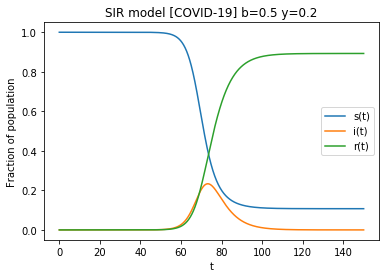
\includegraphics[width=9cm]{covidb12y15.png}
\centering
\caption{COVID-19 in SIR Model for $\beta=0.5$}
\label{fig:covid1}
\end{figure} 


But if we decrease the number of infections to one per 5 days, so the $\beta = 0.2$, then there is no epidemic:

\begin{figure}[ht]
    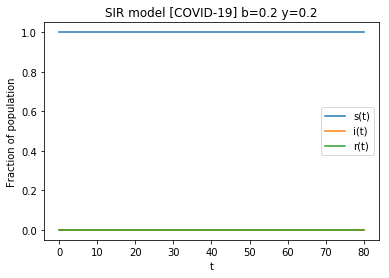
\includegraphics[width=9cm]{covidb15y15.png}
    \centering
    \caption{COVID-19 in SIR Model for $\beta=0.2$}
    \label{fig:covid3}
\end{figure} 

We can easly notice that, the factor determining if the epidemic will happen is the rate of new infections $\frac{di}{dt}$, if it is positive, then there will be epidemic, and if it's negative, people will recover faster than spread of infection, so there will be no epidemic.

We can calculate the value of $\frac{di}{dt}$ in the t0 and check if the value is negative of positive, the negative value mean the decrease of infections from the beginning, so we can be sure that, there will be no infections.

Let's represent the factor determining of the epidemic in form of inequation, which if satisfied, will lead to epidemic

\[i(t) \beta s_0 - \gamma i(t) > 0\]

Since the fraction of infections $i(t)$ is never negative, we can omit it in our inequation.

\[\beta s_0 - \gamma > 0\]
\[ s_0 > \frac{\gamma}{\beta}\]

Here we can introduce $R_0$ as Basic Reproduction Number

\[ R_0 = \frac{s_0 \beta}{\gamma}\]

which represent the number of people, each infected person can infect before being recovered. Thus if $R_0 = 2$ then each infected person can infect on average 2 new people before being recovered, so the number of infections grows exponentially, and if $R_0 = 0.5$, then for each 2 people, only 1 new infection happens, and the number of infections decrease exponentially. $R_0 = 1$ is called $epidemic threshold$ where the number of new infections equals the number of recovers, so the total number of infected people is always the same and equals the initial number of infected people $I_0$. For example, the Basic Reproduction Number $R_0$, for seasonal flu the value is estimated between 0.9–2.1\cite{coburn2009modeling}, whereas for COVID-19 it's estimated to 2.2 in early stage (January) \cite{li2020early} and recently to 5.7 (April) \cite{readeid}.

To decrease the results of epidemic, we can decrease the numbers $s_0$ and/or $\beta$, or increase $\gamma$. Since we have little control over the time of recovery ($\gamma$), the only way to reduce the impact of infection is to reduce the number of contact between infected and suspicious people. That's why, the social distancing is so important in fight with epidemics.


It might be also valuable to know the maximum number of infected people at any given time. We can calculate it by combining the first two parts of SIR differential equations.
\[
\begin{rcases}
\frac{dS}{dt} = - I \beta S \\
\frac{dI}{dt} = I \beta S - \gamma I
\end{rcases}
\]

into 

\[\frac{dI}{dS} = \frac{\beta I S - \gamma I}{\beta I S}\]

which then reduces to 
\[\frac{dI}{dS} = -1 + \frac{\gamma}{\beta S}\]

here we can replace $\frac{\beta}{\gamma}$ by $q$; so called \it{contact ratio}, which is described as fraction of population, that comes into contact with an infected individual, during the period when they are infectious.

\[\frac{dI}{dS} = -1 + \frac{1}{qS}\]

now we can integrate the equation and get

\[I + S - \frac{1}{q} \ln{S}\]

or more precisely

\[I_0 + S_0 - \frac{1}{q} \ln{S}\]

We know that to find the function maximum we need to find the place where its deritive equals zero. And here, the right side of the equation 

\[\frac{dI}{dS} = -1 + \frac{1}{q S}\]

equals to zero, when this equation is satisfied.

\[1 = \frac{1}{q S}\]

which happens when 

\[S = \frac{1}{q}\]

In order to find the maximum value of I, we can replace the $S$ by $\frac{1}{q}$ in the equation

\[I_0 + S_0 - \frac{1}{q} \ln{S}\]

so we get

\[I_0 + S_0\frac{1}{q} - \frac{1}{q} \ln{S\frac{1}{q}}\]

\subsection{SIS Model}

There are some kind of diseses, where the individual can gets infected many times e.g. the flu. For this kind of epidemic, the state flow looks following $S -> I -> S$, hence the name SIS. 
To calculate this kind of model, we need modify the previous equations, that the change $\gamma i(t)$ will go to suspicious state instead of recovery.

\[\frac{si}{dt} = - i(t) \beta s(t) + \gamma i(t)\]

\[\frac{di}{dt} = i(t) \beta s(t) - \gamma i(t)\]






\subsection{Summary}
Unfortunately those modes doesn't fit exactly to our needs, since they are based on the propability that some individual will meet someone else. In our problem, the network is static, our neighbors don't change in time, thus we have to create different model of dissemination spread. 

In our model the infection is the abstract representing trust, so we should take a look how the trust graph are build to understand how we could leverage the mechanisms for our infection spread.




\section{Trust graph}
How are they created ? In life, in networks ? What does it mean to create trust relationship. What do we understand by trust relationship. In environments that or another. 

Then we assume that such relation is already achieved. 
LOCKSS - solve the problem in one way, Wikipedia in another (experts consensus), but they doesn't fit to us, why ?. 

Why do we even look for solution for our problem in the context of human trust ? It turns out that people are still one of the most advanced technology, thus we can get inspired by some of the solutions that worked in human societies for centuries. Let's dive into it.
Yuval Noah Harari in his book "Sapiens: A Brief History of Humankind" states that the most important feature of human language is rumor. Rumor let us know which person is not trustworthy without having to interact with him directly. If our best friend Bob, tells us, that Carlie is theft, we don't need to get stolen to be convinced about it. Same applies in inverse scenario, if Bob tells us, that Carlie sells great quality products, we are now more likely to buy products from him. We notice that each person we know directly or indirectly, gets labeled by some tags. One can be labeled as Helpful, Conscientiousness and also Not-Trustworthy, while other can be labeled as Unhelpful, Lazy but Trustworthy. Here is this paper we are limiting our range of study just to dimension of Trustworthness.
What if we have three friends Alice, Bob, Charlie. Alice and  Bob tells us that David is Trustworthy, while Charlie claims that he's not. Decision of labeling David as Trustworthy or not, requires some kind of decision evaluation algorithm.
One might assume that if there is at least one person who doesn't trust him, there must be something wrong with him, and will label him as Not-Trustworthy. One can use the most natural to human beings evaluator which says, do want majority of people do, thus if Charlie is trusted by majority, I will trust her too. Another one can slightly generalise this evaluator and say that person is trustworthy, only if $\xi$ percentage of my friends trust him. 

At this point it's worth introducing some convention. When we say friend we mean a trustworthy person, in other words, person to who we have trust relation to. Let $N$ to be a set of all considered person group, friends and non-friends. Let $F$ be a set of all our friends $f \in F$. Let $F_n$ be a subset of $F$ where all $f$ trust person $n$. Then we will call $\%_n = |F_n|/|F|$ the proportion of our fiends who trust particular person $n$. Let's call $\xi$ (where $0 \le \xi \leq 1$) the minimum proportion of our friends $\%_n$ who needs to trust person $n$ in order to make me trust him. 

So as we said previously that we will trust David only if majority of our friends trust him. We denote trust function as $T(n) = \%_n > \xi : (N) \rightarrow \{0,1\}$. 
Let's use this formula to evaluate if $David$ is trustworthy person. Let $\xi = 0.5$. We know that Alice and Bob do trust David, while Charlie don't.
\[T(David) = \%_{David} > \xi\]
\[= |F_n|/|F| > \xi\]
\[= \frac{2}{3} > \frac{1}{2}\]
\[= 1\]
Then it turns out that $David$ is \textbf{Trustworthy}


People with low $\xi$ easly gets manipulated, we call them naive.
People with high $\xi$ hardly gets convinced, we call them stubborn. 

Another generalisation might be adding weights to this evaluator, let's say that Charlie is our brother, while Alice and Bob are our cousins, and we trust 3 times stronger to our brother than cousin. Let's call $W(f): (F) \rightarrow \Re$ the function that maps our friend to the weight of how strong we trust him. In this case weighted proportion of our friends \[\%_n = \frac{\sum\limits_f^{F_n} W(f)}{\sum\limits_f^{F} W(f)}\]

When we assume weights $W(Alice) = 1, W(Bob) = 1, W(Charlie) = 3$, and $\xi = 0.5$. We can calculate weighted proportion $T(David)$ as follows:
\[T(David) = \%_n > \xi\]
\[= \frac{\sum\limits_f^{F_n} W(f)}{\sum\limits_f^{F} W(f)} > \xi\]
\[= \frac{\sum \{1,1\}}{\sum\{1,1,3\}} > \frac{1}{2}\]
\[= \frac{2}{5} > \frac{1}{2}\]
\[= 0\]
Then it turns out that $David$ is \textbf{Not-Trustworthy}

But this view is based on static network of connections. We somehow meet Alice, Bob and Charlie, and we gets convinced about their trustworthness. Thus there must be a second way of gaining our trust. Let's modify our trust function by allowing External Trust Obtaining(ETO). $T(n) = \%_n > \xi \lor ETO(n) : (N) \rightarrow \{0,1\}$. 

Another think we can observe in the context of trust network is time. Should we still trust our friend from elementary school if we haven't seen him for decades ? We argue that trust is function of time.

// How to continue from trust graph subchapter 



We said that infected node trusts the content published by the publisher, therefore the user who request the content from such "infected" node is convinced that the content can be trusted. In current scheme 

In current schema, the malicious publisher can infect partial population of nodes, 



 The infection is started by the publisher (honest or not) who publish the first proo-of-time certificate to the home node. Home node is assumed to be assigned to each publisher, do he can not choose arbitrary node. 


Content Publisher who is trying to convince the network that can publish the proof-of-time certificate to one of the nodes, 

Overlay Network of trust

For further research, we need some graph models, that we will base our proof-of-time mechanism on. We can not be sure how the structure of ICNetworks will look like, neither assume that the overlay network of trust match it. We want to allow any arbitrary trust graph structures to be build on top of it. Let's investigate how the trust graph can be created. 

Therefore we need to reach the researches from other types of networks. We can losely assume that the structure of ICNetwork will match with the structure of current internet - more precisely internet Autonomous Systems. Yet, we think that the overlay trust network should be independent from the physical structure.  That way, we can allow to create any arbitrary trust graph. It turns out that the structure of internet and structure of social networks shares common distributions called power-law. 

it allows us to create any arbitrary graph  Fortunately we know that structure of internet and social networks share common distributions, called scale-free that satisfies power-law distribution. 




%\section{Blockchain}
%When we speak about trust, openness and decentralization it's always worth to consider Blockchain technology. Here we will try to use Blockchain to achieve previously stated requirements. Some of the properties Blockchain technology gives us are: immutability - once written, data can not be modified. Time assurance - each block is published in apprx. 10min. This feature gives us a clock that will provide us signed timestamps. Sign ensure trust based on consensus settled by proof-of-work algorithm.

\section{Proof of Time - Abstract solution}
We propose system where authentication is based on \textit{proof of time} access to private keys. 
We noticed that the proof-of-time must be published in either neutral place or in verifier place. So the publisher can not use it's influence to modify the data. 







\section{Stolen Credentials Problem}
How long on average does it take to detect stolen credentials on average.

\section{Graph Burning}
How does it differ from out solution ? Where to place fire so it burn as fast as possible ?


\section{Graph Infections - Concrete solution}
Proposition \cite{jekon2019content}
Simulator \url{https://github.com/stasbar/MASTI}

The graph we are considering is limited only to one content at a time. So we can assume that all nodes in the graph are interested in such content trust.

\section{Bitcoin - naive solution}
In previous section we discussed solution based on graph infections. Here we will propose naive solution based on one of the core features of Bitcoin Blockchain, precisely on probabilistic fixed interval between blocks creation. In bitcoin protocol, transactions are stored in data structure called Blockchain. Each node in p2p Bitcoin network can participate in block creation process called mining, this becoming miner. Each node becomes validator of new transactions that gets to Bitcoin network. follows strict rules that 

\section{Blockchain - Concrete solution}
We could use Bitcoin blockchain, or any other blockchain with constant time block creation, to persist proof-of-time claims. In Bitcoin each block is created in appx. 10min. We could take advantage of it, as a global, secure signing clock. Each new block has it's own unique hash, which can be used as a signing key. For our proof-of-time claims, or better we could persist our claims inside blockchain itself. Naive approach would be to send a empty (just fee) transaction from publisher account to hash of the content address. This way everyone can check, the history of hash of the content. Ensuring that it was proven by publisher for long enough. Of course this approach is conceptual. Bitcoin network is not suitable to operate in for network devices. Therefore we will outline the properties especially interesting in blockchain, and try to find out another blockhain or propose our own design. We consider Blockchain in first place, mainly because it's secure. Secure in terms of Byzantine Fault Tolerant system, but also as immutable storage. Not one can change the previously written data, without recalculating the proof-of-work puzzle, and overtaking rest of the network in computational power competition. This mechanisms works great for blockchains that servers store of value purposes. Our needs are completely different, we need a system that is asymptotic secure, so no (more powerful) node can overtake the whole network. That way, we lose the property of ~10min period ticking clock. We also can not incentivese nodes to behave honest by staking electrical power. We also need to get rid of fees since the Internet protocol on this level must be free. Therefore we need to protect from DoS attack in different way. Another important properties are openness and scalability. We need to design system that allow joining new participants and is highly scalable, otherwise we are limiting the protocol to special use cases, rather than global Internet protocol. Such software needs to operate on network devices which are resources constrained. Thus it needs to be lightweight, both in computational power and memory consumption.

Our solution to this problem is modification of \cite{jekon2019content}, by adding Blockchain as a storage, and modifying consensus algorithm.

Each publisher who wants to publish the content to the network, must start with its home node. That node, create transaction in which he certifies the content proved by the publisher. Such certificate is then flooded to whole network, so they can update the current state of trust to the content. After some delay (clock tic), such node also create certificate in which he point to the one of neighbours node which can be infected next, where the publisher is also allowed to publish the content. The next node will accept the infection only if he is an home publisher, or if he is pointed as the next node by the previous node. Publisher show valid certificate (signed by previous node, and by himself - proving access to private key). Each node can create certification only once per content. 

That way, each node control the time of infection dissemination. If any node notice, that, the new certification was published earlier than previous certification + some fixed delay, it can assume that such node is cheating, and filter the certifications from such node.

Therefore we constructed new consensus algorithm where each node spread infection only if:
- didn't spread the infection for such content before
- previous time of infection was x time ago
- it is the home publisher or contains authorization token issued by some neighbour pointing to the node.

\section{Fusion - Graph infection blockchain based scheme}
We notice that, the chain of approval can be threat like a blockchain. Consensus mechanism here is based purely on each node. Each node control the time delay of the next block. If some node block the transaction, or sends it faster than designed (malicious actor), we can distrust that node. Each external publication create next block. Publisher is responsible for extending that chain to the length of acceptable trust to that content.

\section{Comparison}
\begin{table}[]
\begin{tabular}{lll}
                                   & Graph Infections & Blockchain \\
Byzantine tolerant system          & False            & True       \\
Determined                         & False            & True       \\
Memory expensive                   & True             & True       \\
Progressive trust                  & False            & True       \\
Transport layer dependent          & True             & Optional   \\
Require Network topology awareness & True             & False     
\end{tabular}
\end{table}


\section{Discussion}

\bibliographystyle{plain}
\bibliography{refs}

\end{document}

